\documentclass[11pt,a4paper]{article}
\usepackage[utf8]{inputenc}
\usepackage[T1]{fontenc}
\usepackage{amsfonts}
\usepackage[french]{babel}
\frenchbsetup{StandardLists=true} % à inclure si on utilise \usepackage[francais]{babel}
\usepackage{enumitem}
\usepackage{amssymb}
\usepackage{amsmath}
\usepackage[left=2cm,right=2cm,top=2cm,bottom=2cm]{geometry}
\usepackage{multirow}
\usepackage[dvipsnames]{xcolor}

\usepackage[T1]{fontenc}
\usepackage{fouriernc}
\usepackage{graphicx}

\usepackage{setspace}
\singlespacing
\setlength{\parindent}{0pt}

\usepackage{multicol}
\setlength{\columnseprule}{1pt}

\usepackage{tikz-osci}

\usepackage{fancyhdr}
\pagestyle{fancy}
\renewcommand\headrulewidth{1pt}
\fancyhead[L]{Lycée Denis Diderot }
\fancyhead[R]{Classe de Première}
\setcounter{page}{1}\fancyfoot[C]{page \thepage}
\fancyfoot[R]{Année 2025 2026}
\fancyfoot[L]{Alexis RUIZ}
\usepackage{multirow,tabularx,booktabs}
\newcommand{\cadreblanc}[1]{%
\medskip\framebox[\linewidth][c]{%
\rule{0mm}{#1mm}}\par
\medskip}

\renewcommand{\arraystretch}{2}
\newcommand*\acocher{\quitvmode{\fboxsep0pt \fboxrule0.8pt \fbox{\vrule height1.8ex depth.1ex width0pt \vrule height0pt depth0pt width1.9ex }}}

\AtBeginDocument{\shorthandoff{;}}
\begin{document}
\begin{center}
\vspace{-3mm}
\LARGE{Fiche Méthode} \\

\vspace{2mm}
\normalsize
Déterminer graphiquement la tension maximale et la période d'une tension alternative sinusoïdale.
\vspace{2mm}
\end{center}
\hrule

\begin{minipage}{0.6\textwidth}
La valeur de la tension maximale $U_{\text{max}}$ est égale à 3,5 V

\textbf{Unités :}
\begin{itemize}
\item Abscisse : 1 carreau $\rightarrow$ 2 ms
\item Ordonnée : 1 carreau $\rightarrow$ 1 V
\end{itemize}

La valeur de la période $T$ peut se lire en différents endroits de la représentation graphique.

Ici $T = 4 \times 2 = 8$ ms $= 8 \times 10^{-3}$ s
\end{minipage}
\hfill
\begin{minipage}{0.35\textwidth}
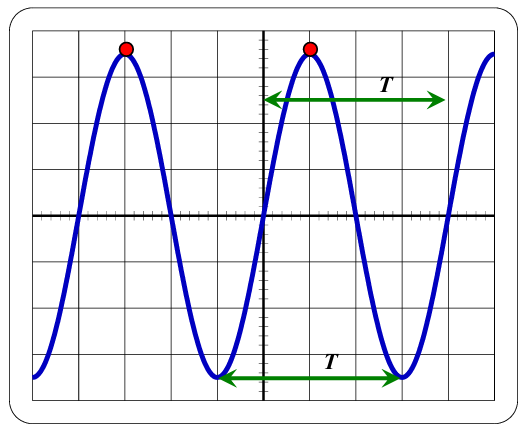
\includegraphics[width=\textwidth]{images/lecture.png}

\end{minipage}

\subsection*{Exercice d'application}

\begin{minipage}{0.45\textwidth}
\centering
\osci[%
scale=0.5,
second channel=0, %1 pour activer la deuxième voie, 0 sinon.
screen offset one=0, %Décalage vertical de la voie 1 sur l’écran
screen offset two=0, %Décalage vertical de la voie 2 sur l’écran
time div=0.5, %Durée par division (en ms)
voltage div one=2, %Tension par division (en V) pour la voie 1
voltage div two=2, %Tension par division (en V) pour la voie 2
sample rate=200, %Taux d’échantillonnage
xy mode=0, %1 pour l’activer, 0 sinon 
func one=4*sin(2*180/0.00250*x),
%func two=3*sin(2*180/0.020*x), 
color one=003399, %Couleur de la voie 1 (en hexadecimal)
color two=1053AF, %Couleur de la voie 2 (en hexadecimal)
graph back color=FFFFFF,
info back color=D6D6D6,
info text color=000000,
main axis color=000000,
grid color=CCCCCC
]
\vspace{-0.3cm}
\begin{align*}
U_{\text{max}} &= \ldots\ldots\ldots\ldots\ldots\ldots = \ldots\ldots\\
T &= \ldots\ldots\ldots\ldots\ldots\ldots = \ldots\ldots
\end{align*}
\end{minipage}
\hfill
\begin{minipage}{0.45\textwidth}
\centering
\osci[%
scale=0.5,
second channel=0, %1 pour activer la deuxième voie, 0 sinon.
screen offset one=0, %Décalage vertical de la voie 1 sur l’écran
screen offset two=0, %Décalage vertical de la voie 2 sur l’écran
time div=0.5, %Durée par division (en ms)
voltage div one=5, %Tension par division (en V) pour la voie 1
voltage div two=2, %Tension par division (en V) pour la voie 2
sample rate=200, %Taux d’échantillonnage
xy mode=0, %1 pour l’activer, 0 sinon 
func one=17*sin(2*180/0.002*x),
%func two=3*sin(2*180/0.020*x), 
color one=003399, %Couleur de la voie 1 (en hexadecimal)
color two=1053AF, %Couleur de la voie 2 (en hexadecimal)
graph back color=FFFFFF,
info back color=D6D6D6,
info text color=000000,
main axis color=000000,
grid color=CCCCCC
]
\vspace{-0.3cm}
\begin{align*}
U_{\text{max}} &= \ldots\ldots\ldots\ldots\ldots\ldots = \ldots\ldots\\
T &= \ldots\ldots\ldots\ldots\ldots\ldots = \ldots\ldots
\end{align*}
\end{minipage}

\vspace{0.2cm}

\begin{multicols}{2}

\subsection*{Relations entre $U_{\text{max}}$ et $U$}

\begin{equation*}
U = \frac{U_{\text{max}}}{\sqrt{2}} \quad \text{ou} \quad U_{\text{max}} = U \sqrt{2}
\end{equation*}

La relation n'est valable que pour une tension sinusoïdale

\vspace{0.3cm}

$U_{\text{max}}$ est la \underline{\hspace{5.8cm}} d'une tension sinusoïdale.

$U$ est la \underline{\hspace{6cm}} d'une tension sinusoïdale.

Elle est mesurée par un \underline{\hspace{3.8cm}}

\vspace{0.8cm}

\subsection*{Relations entre $T$ et $f$}

\begin{equation*}
T = \frac{1}{f} \quad \text{ou} \quad f = \frac{1}{T}
\end{equation*}

$T$ est la \underline{\hspace{2cm}} de la tension sinusoïdale en \underline{\hspace{2cm}} \\


$f$ est la \underline{\hspace{3cm}} de cette même tension. \\[3mm]

Elle s'exprime en \underline{\hspace{3cm}}

\end{multicols}

\vfill 
%\subsection*{Exemples}
\begin{multicols}{2}
\textbf{Exemple 1 :} calcul de $U$ pour $U_{\text{max}} = 25$ V :
\begin{equation*}
U = \frac{U_{\text{max}}}{\sqrt{2}}  = \hspace{3.5cm}  \text{ (arrondir à 0,1)}
\end{equation*}

\textbf{Exemple 2 :} calcul de $U_{\text{max}}$ pour $U = 240$ V :
\begin{equation*}
U_{\text{max}} = U \sqrt{2} = \hspace{3cm}  \text{ (arrondir à 0,1)}
\end{equation*}

\textbf{Exemple 3 :} si $f = 500$ Hz alors
\begin{equation*}
T = \frac{1}{f}  = \hspace{7cm} 
\end{equation*}

\textbf{Exemple 4 :} si $T = 15$ ms $= 15 \times 10^{-3}$ s alors
\begin{equation*}
f = \frac{1}{T} = \hspace{5cm}  \text{ (arrondir à l'unité)}
\end{equation*}
\end{multicols}
\vfill 




\end{document}